\chapter{Methods for the analysis of Dynamics of Temporal Relationships of Neural Activities Using Noisy Optical Imaging Data}	
\label{chap:analysis}
\section{Methods}


The first step in scientific investigation is usually the collection of data. Once the data is collected it needs to be analysed and processed to allow for interpretation within the context of what is already known. \ac{VSD} data allow us to record intracellularly from significantly more neurons at the same time than what electrophysiological techniques allow us to record but at the same time the data is more noisy and thus need different methods for analysis. In the next sections we discuss the methods we have devised for the analysis of injected and bath-applied \ac{VSD} to the \ac{STG} of the brown crab (\species{Cancer pagurus})

The dynamics of the temporal relationship of the activities of neurons forming neural circuits is critically important for the flexible and adaptive delivery of the functionality of the circuits \cite{Harris-Warrick1992,Galan2004,Hill2012,Bruno2015}. For example, switching between synchronised and de-synchronised patterns of activity of neurons forming functional circuits in the hippocampus plays a fundamental role in memory formation, maintenance and recall in vertebrate brains \cite{Axmacher2006,Robbe2006}. In the case of epilepsy a switch to excessive synchronisation of neural activities breaks down the functionality of many neural circuits and the neural systems formed by them \cite{FeldtMuldoon2013, Engel2013}. Recently it has been shown that the fine timing of inputs to different parts of the dendritic tree of neurons in the visual cortex of mammals determines the actual receptive field of the neuron \cite{Chen2013}. In general, both relatively simple and complex changes in the temporal relationship of neural activities can play a critical role in the delivery of the functionality of neural circuits.

While multi-electrode arrays allow recording of many individual neurons in artificially created cell culture \cite{Potter2001, Spira2013}, the activity of neurons in such context is not truly comparable to the activity of neurons in real physiological conditions. In other settings, when multi-electrode array or multiple multi-electrodes (e.g. tetrodes) are used to record many neurons from brains or brain slices in physiological conditions, the connectivity between the recorded neurons is usually not known \cite{Guitchounts2013, Scholvin2015, Santos2012}. the impact of this is that a large part of the work on neuron resolution dynamics of neural circuits remained mostly theoretical \cite{Schneidman2006, Shlens2006, Paninski2010}.

Currently used techniques of optical recording of neural activity using voltage-sensitive dyes and calcium dyes allow high spatio-temporal resolution recording of the activity of many neurons, making possible the study of the dynamics of temporal relationships of neural activities in biological neural circuits \cite{Canepari2010}. While many applications of these techniques are used to record many neurons that are not necessarily directly coupled synaptically \cite{Mukamel2009, Rothschild2010}, it has been shown that these methods can also be applied successfully to a range of biological neural systems to record the activity of many synaptically coupled neurons simultaneously. These techniques have been applied to analyse the functionality of neurons in leech ganglia \cite{Briggman2010}, to study the dynamical assignment of functional roles to neurons in snail ganglia \cite{Hill2012, Bruno2015}, to record almost simultaneously the activity of all neurons in the brain of the zebra fish embryo \cite{Ahrens2012}, to analyse the activity of neurons in intestinal neural ganglia in guinea pigs \cite{Obaid1999}, and to study the activity of synaptically coupled neurons in the stomatogastric ganglion of crabs \cite{Stein2011, Staedele2012}.  However, it should be noted that usually the recorded data is quite noisy, potentially making its analysis difficult.
	
	
\section{De-trending and Event Triggered Averaging}
\label{sec:detrend}
The different types of neurons of the \ac{STG} can be identified by intracellular recordings. Each type of neuron has a distinct shaped voltage waveform that it produces. To confirm the identification of the neuron the voltage waveform is also correlated to extracellularly recorded spikes from the motor nerves. When using \ac{VSD}, the identification of the neurons are more difficult due to baseline drift and noise obscuring the wave forms.  A \ac{VSD} recording is seldom clear enough to discern any spikes. It is, however, possible to obtain a voltage wave form good enough for identifying the recognisable wave features of a specific neuron by first de-trending and then averaging the captured data.

\begin{figure}[H]
	\centering
		\includegraphics[height=17cm]{graphics/ident_neurons.png}
		\caption[Identifying pyloric \ac{CPG} neurons.]{\textbf{Identifying pyloric \ac{CPG} neurons.} Neurons of the pyloric \ac{CPG} can be identified by features of the voltage waveform as well as correlating the waveform to extracellularly recorded spikes from motor nerves. The voltage waveforms of the \acp{PY}, \acp{PD}, \ac{LP} and \ac{VD} are shown here. The horizontal shaded line correlates the waveform with extracellular recordings that were made over the \ac{lvn} and \ac{mvn}. The red arrow points to features typical of the specific neurons \footnote{From the Nadim, Golowasch, Bucher STG website at \url{http://stg.rutgers.edu/resources/Cancer_Guide.pdf}.}. Recording such as these are made using electrophysiological techniques.}
		\label{fig:ident_neurons}
\end{figure}

A trend in a time series is gradual change in some property of the the series of the time interval under investigation. During recordings with \acp{VSD} a decaying trend can often be observed, which can be attributed to dye bleaching \cite{Briggman2010}. 

De-trending on data was done with an R implementation of the following equation which uses a linear approximation of $x_{t}$ as a function of time:

\begin{equation}
\label{eq:detrend}
(m_{i}^{*},b_{i}^{*}) = \frac{argmin}{m,b}\sum_{t=i}^{i+w}\|x_{t}-m\cdot(t-i)-b\|^{2} 
\end{equation}

\begin{equation}
\begin{array}{c c }
y_{i}=x_{i}-m_{i}^{*}\cdot i - b_{i}^{*} \nonumber
\\
i=1,\ldots,z \nonumber
\end{array}
\end{equation}

where:

$m$ is the slope of the linear approximation.

$b$ is the bias or y-intersection of the approximation.

$w$ is the chosen window size.

An appropriate window size needs to be chosen for de-trending. The result of applying equation \ref{eq:detrend} to a recording can be seen in figure \ref{fig:baseline_drift}.

\begin{figure}[H]
	\begin{center}
		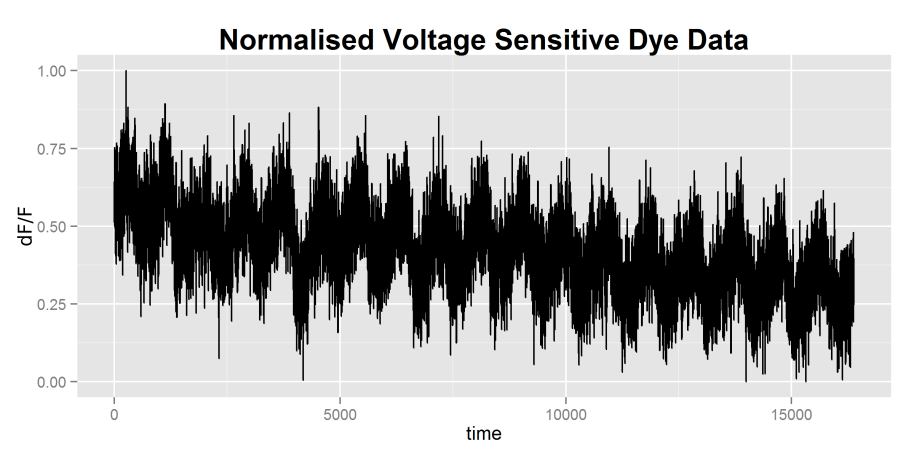
\includegraphics[width=\textwidth]{graphics/data_trending.png}
		\label{fig:trending}
		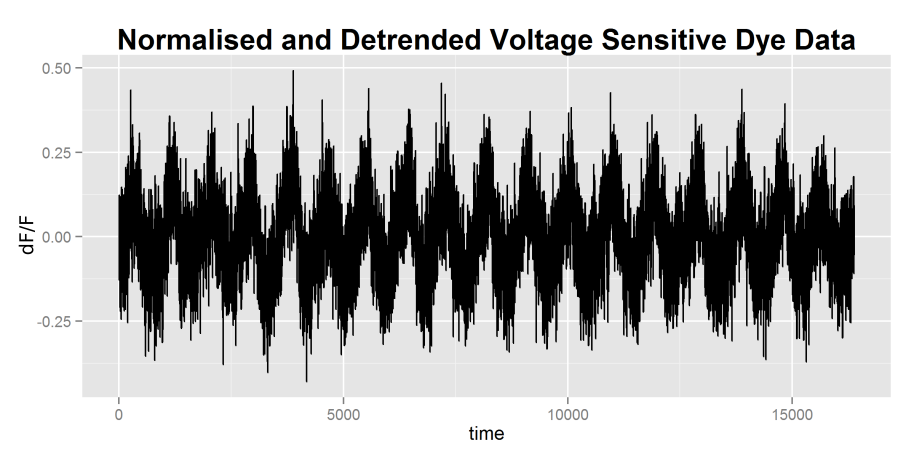
\includegraphics[width=\textwidth]{graphics/data_detrend.png}
		\label{fig:detrending}
		\caption[Neural activity before and after detrending.]{\textbf{Neural activity before and after detrending.} Top: Normalised raw data series from voltage dye imaging without detrending. Bottom: Data series after detrending.}
		\label{fig:baseline_drift}
	\end{center}
\end{figure}

After de-trending averaging over phases of the rhythm has to be done. Averaging requires an extracellular recording that can be used to determine the beginning of each phase. The identification of phases has to be done manually by looking at the trace and noting the time stamp of the first spike in a phase. Spike2 software was used for doing the identification as it allows one to zoom in on a trace to find an accurate time stamp. Figure \ref{fig:data_phases} shows an extracellular recording of the pyloric rhythm made over the \ac{dvn}. The vertical red lines indicate the beginning of each phase. The time values of the occurrence of the first spike of each phase is noted.

\begin{figure}[H]
	\begin{center}
		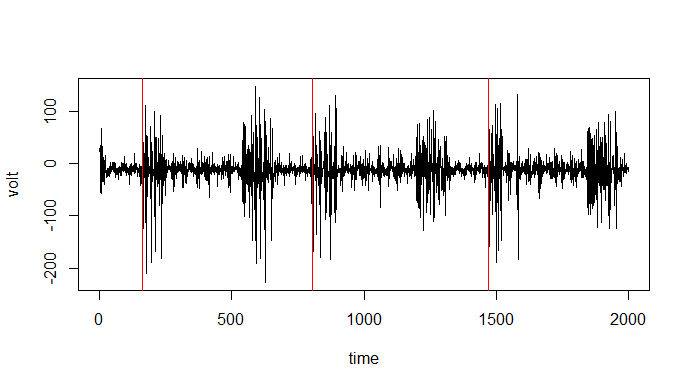
\includegraphics[width=0.8\textwidth]{graphics/data_phases.png}
		\caption[Extracellular recording of the pyloric rhythm.]{\textbf{Extracellular recording of the pyloric rhythm made over the \ac{dvn}}. The vertical red lines indicate the beginning of each phase. The time values of the occurrence of the first spike of each phase is used for doing averaging of the phases. Shown here are only three phases but as many phases as possible should be identified for more accurate averaging.}
		\label{fig:data_phases}
	\end{center}
\end{figure}

At this point it is necessary to decide over how many phases the averaging needs to be done. Let us call the number of phases $p$. Typically, for this research, the decision was made to average over three phases as averaging artefacts on the first and last phase often made them unsuitable for use. Three phases proved to be adequate to identify a neuron against the extracellular recording and also gives enough information for further analysis as described in the following text. Starting at the beginning of each identified phase, the data are placed in arrays, where each array contains $p$ phases. The phases are never exactly the same length, making it necessary to find the length, in time units, of the shortest array of phases. Let us call the length of the shortest phase $l$ and $a$ the number of arrays that can be extracted from the data. If $n$ is the number of phases identified then the number of arrays will be:

\begin{equation}
a=n-p+1
\end{equation}

at each time unit in each array, sum the value of the time points and divide by the number of arrays (see figure \ref{fig:averaging}) to give an average for that time point. Averaging is done up to the length of the shortest array ($l$).  The fact that the arrays are not the same length accounts for the artefacts that are sometimes observed in the last phase which can make it unusable. 

\begin{figure}[H]
	\begin{center}
		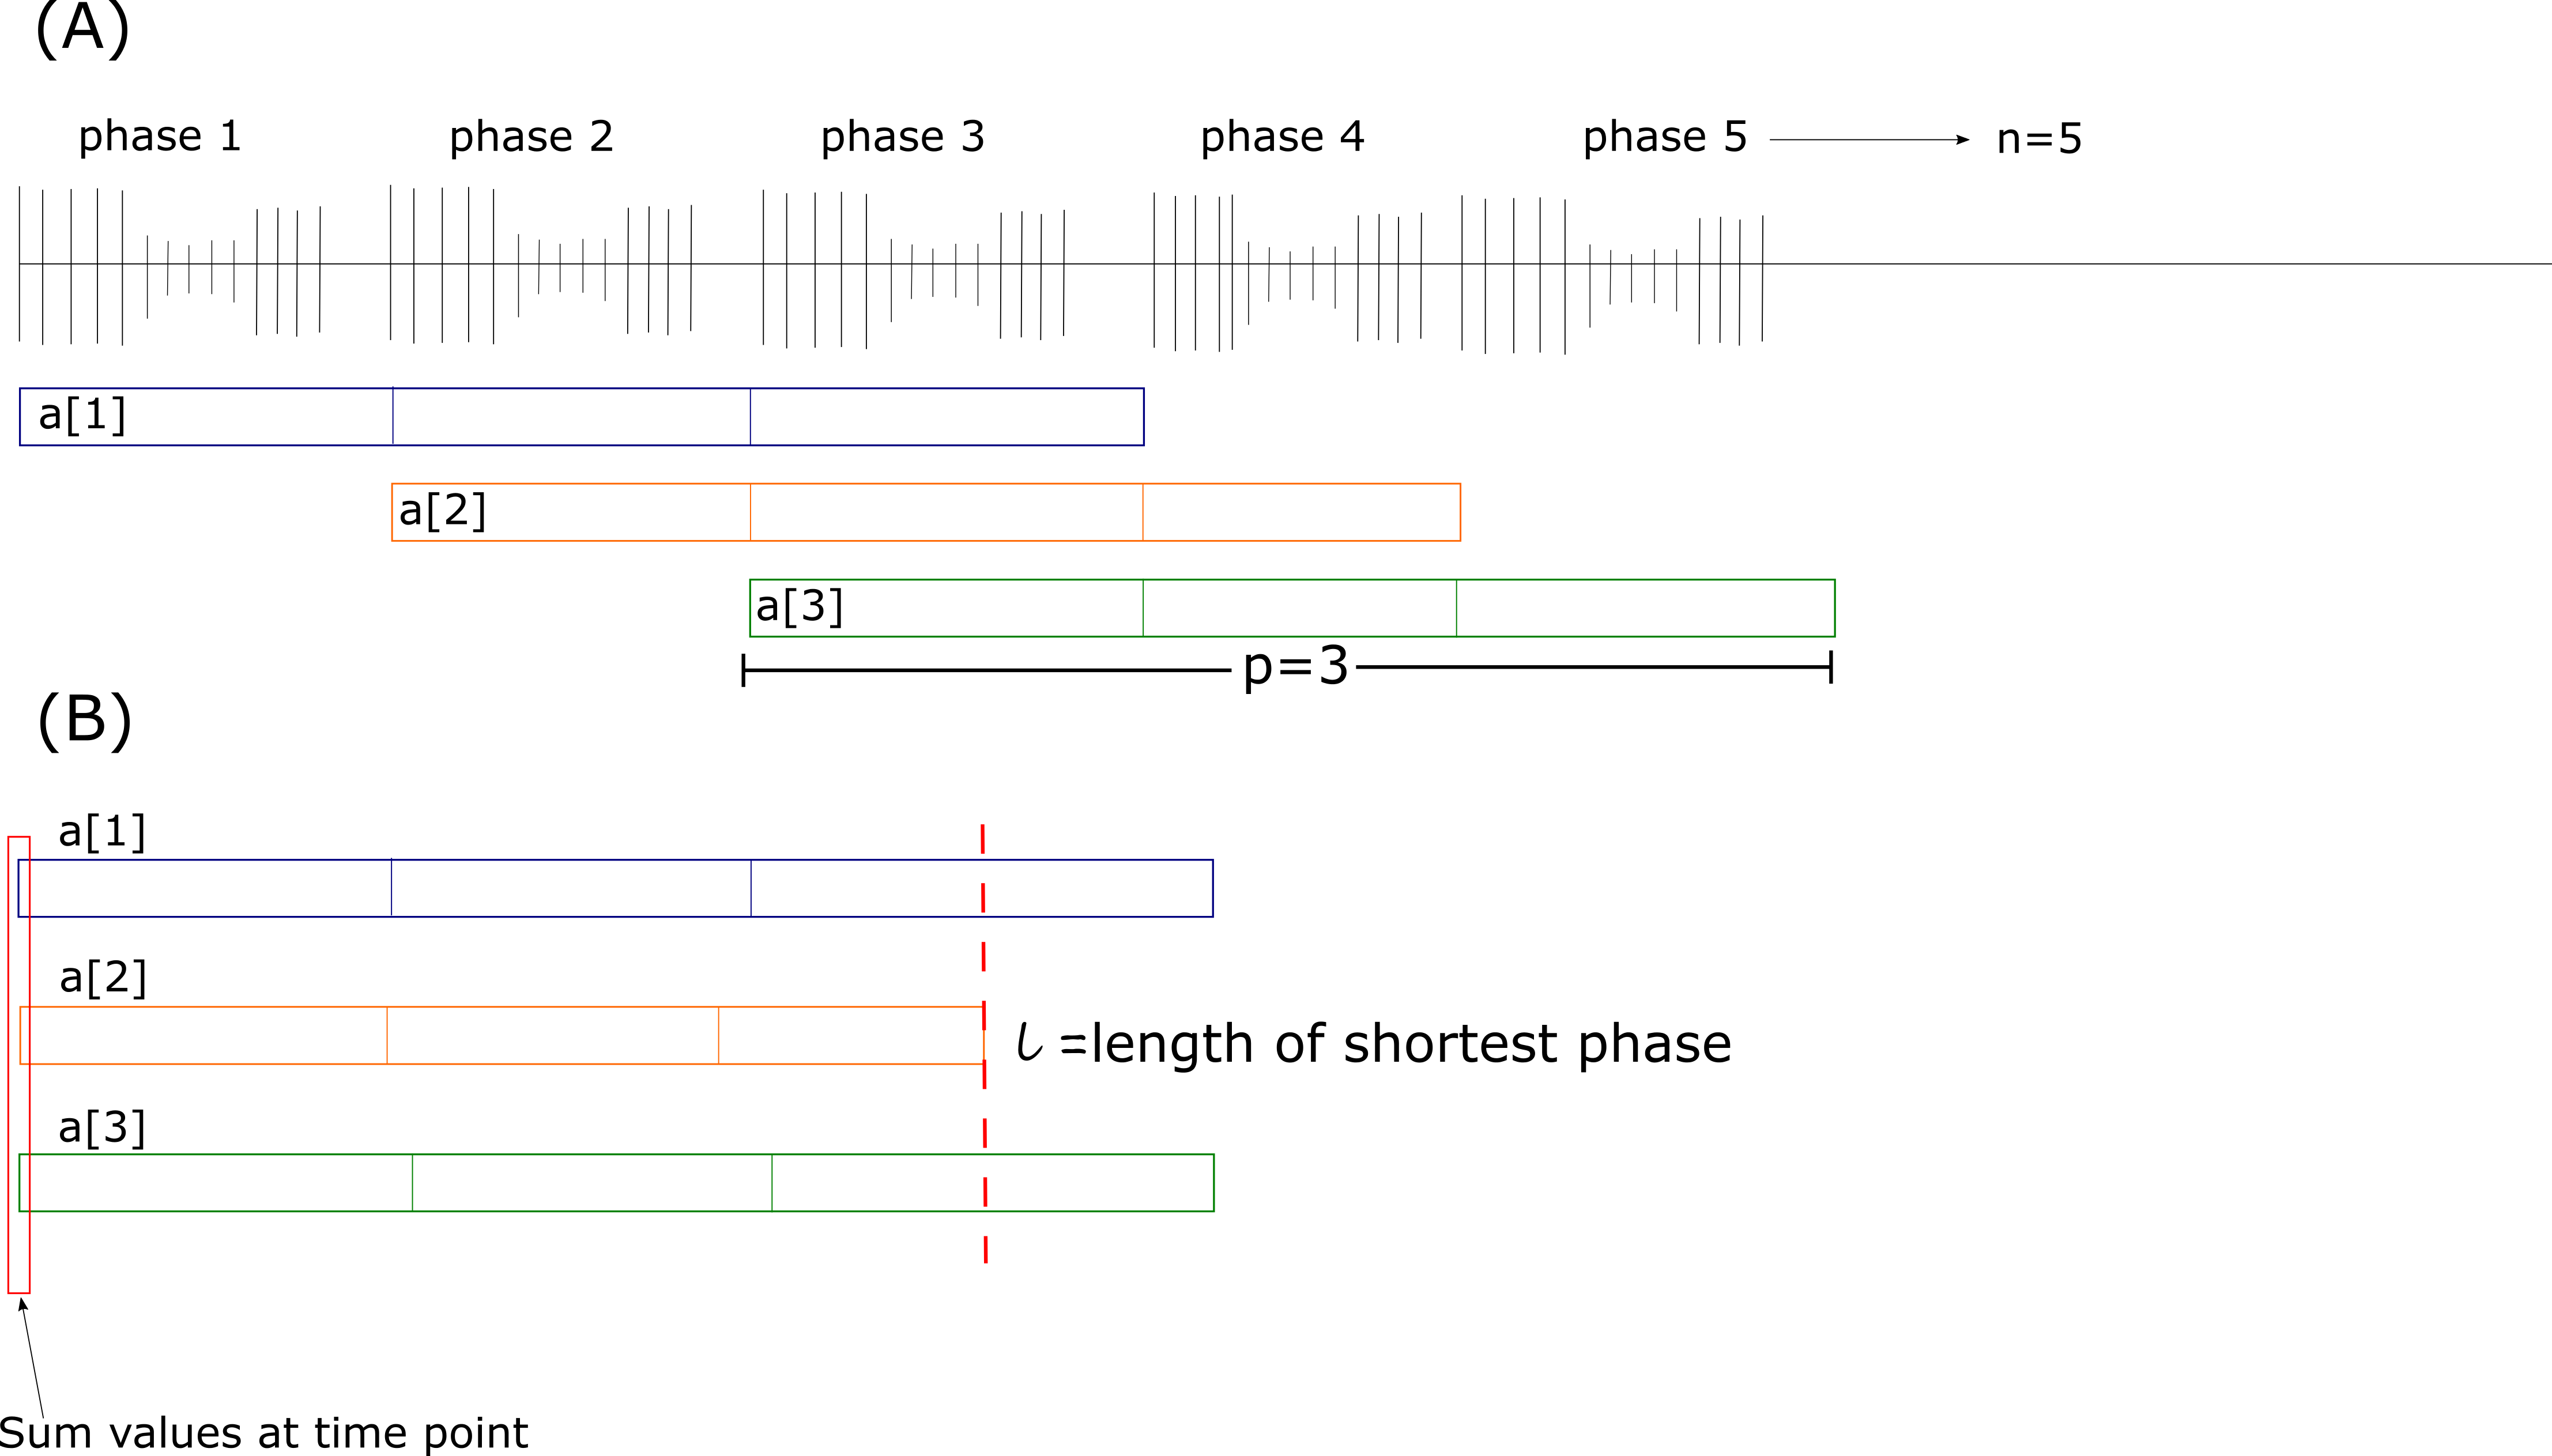
\includegraphics[width=\columnwidth]{graphics/averaging.png}
		\caption[Event-triggered averaging.]{\textbf{Event-triggered averaging.} (A) illustrates the identification of phases in a time series. Five phases are identified (n=5) in this example. The data are placed in arrays where each array contains $p$ phases (p=3). (B) illustrates the summing of each time point over all the arrays. The sum is then divided by the number of arrays to get the average for that time point. This averaging is done for all time points up to the length of the shortest array ($l$), indicated by the dotted red line. }
		\label{fig:averaging}
	\end{center}
\end{figure}

Figure \ref{fig:averaged} shows an averaged time series. This averaging methods works well for both intra- and extracellularly applied \ac{VSD} recordings. 
\begin{figure}[H]
	\begin{center}
		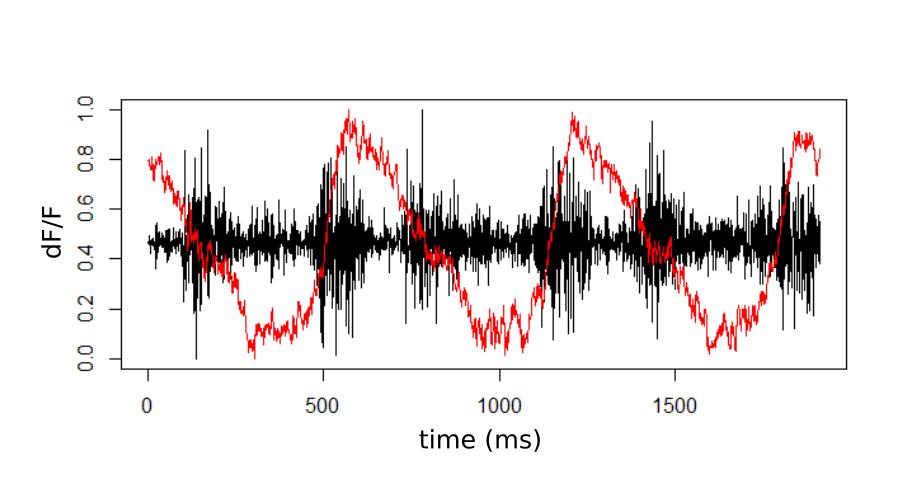
\includegraphics[width=\columnwidth]{graphics/averaged.png}
		\caption[Averaged intra- and extracellular recording.]{\textbf{Averaged intra- and extracellular recording.} The black trace shows an extracellular recording averaged over three phases. The red trace is the averaged data from figure \ref{fig:baseline_drift} overlaid onto the extracellular recording, illustrating the correlation of the voltage sensitive dye recording with the extracellular recording and how the shape of the wave becomes apparent after averaging. To be able to overlay the data as in this figure, it is necessary to normalise both traces. In this case, normalisation was done to values between 0 and 1.}
		\label{fig:averaged}
	\end{center}
\end{figure}

\section{Analysis of Noisy Optical Imaging Data}
\label{sec:analysis_methods}

Using the \ac{VSD} imaging techniques described in section \ref{sec:vsd} the \ac{STG} was first imaged in normal saline. For the purpose of dopamine exposure the \ac{STG} was perfused with saline containing dopamine. First a saline solution containing $10^{-6}M$ concentration dopamine was applied to the \ac{STG} for 20 minutes. This condition is called the ``low dopamine'' condition. After the initial 20 minute exposure to dopamine, perfusion with the dopamine saline solution was maintained while imaging. Next, a saline solution containing $10_{-4}M$ concentration dopamine (i.e. 100 times more dopamine than in the previous experimental condition) was used and the \ac{STG} was exposed to this for 20 minutes. This condition is called the ``high dopamine'' condition. The preparation was imaged again while perfusion with the high dopamine saline solution is maintained.

The activity of neurons participating in biological neural circuits follows various patterns. Some neurons are silent most of the time balancing around their resting potential, on occasion firing a single or a few spikes, for example many cortical neurons in mammals \cite{Brumberg2000}. Other neurons, such as invertebrate neurons that form central pattern generators, periodically generate bursts of activity \cite{Harris-Warrick1992}. One relatively common feature of the various neural activities is that, generally, the spiking of neurons (especially multiple spikes) happens on the top of a depolarization plateau (fig \ref{fig:spikes}). 

\begin{figure}[H]
	\begin{center}
		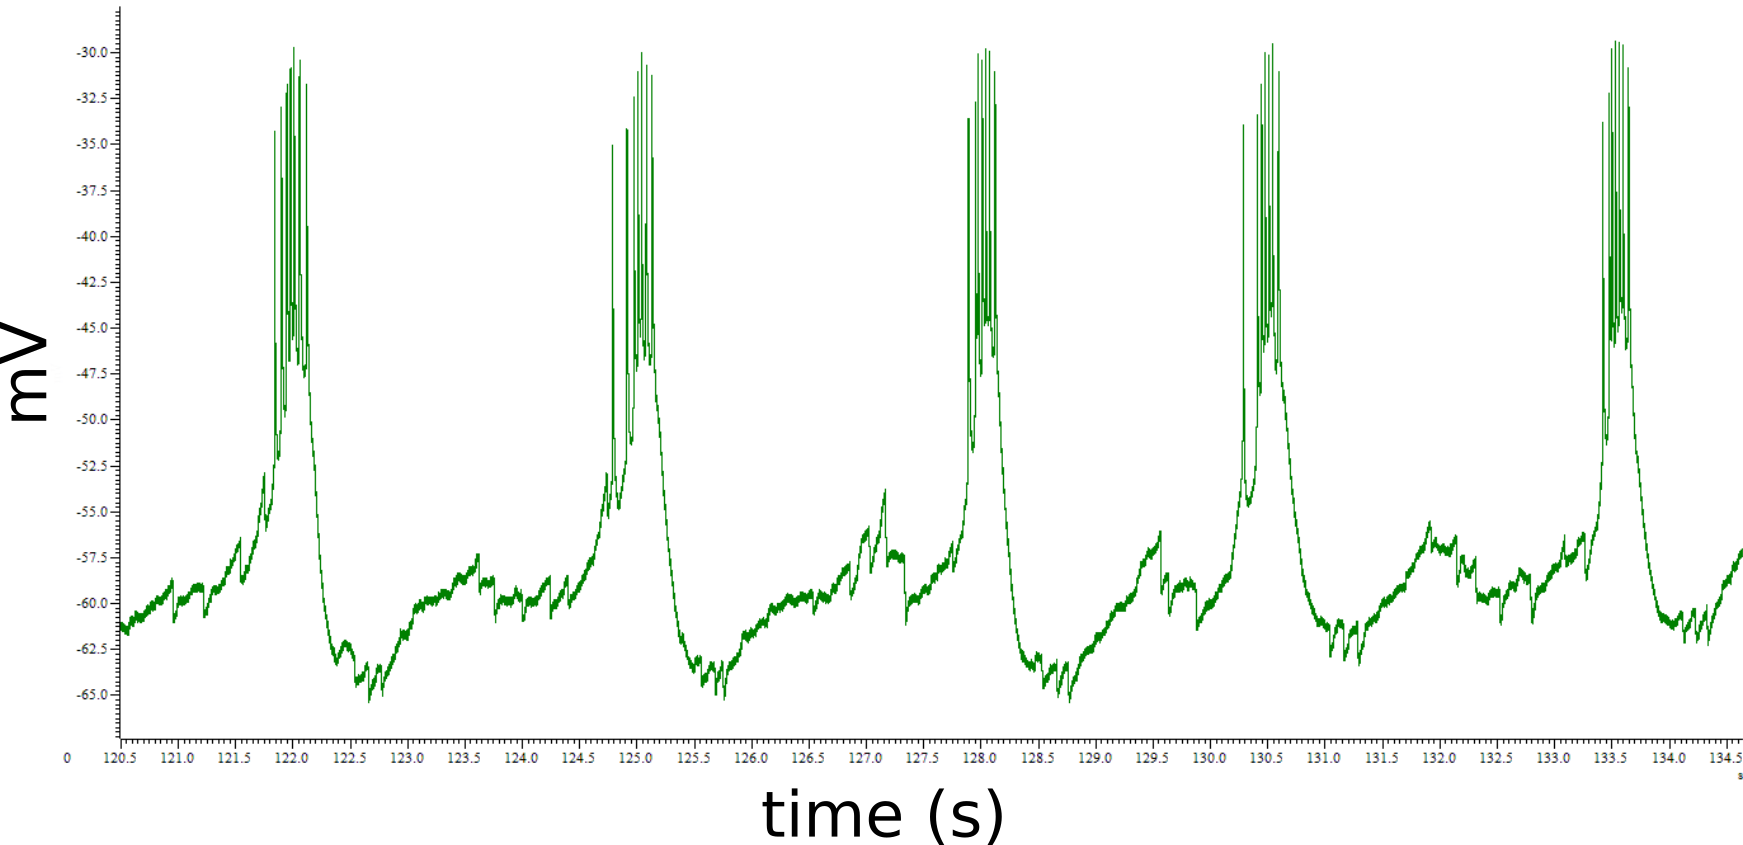
\includegraphics[width=\columnwidth]{graphics/PD_intra.png}
		\caption[Intracellular recording of \ac{STG} neuron.]{\textbf{Intracellular recording of \ac{STG} neuron.} Intracellular recording of a neuron from the crab stomatogastric ganglion. The spiking of neurons (especially multiple spikes) happens on the top of a depolarization plateau.}
		\label{fig:spikes}
	\end{center}
\end{figure}

In some cases the amplitude of membrane potential difference deviations during the spikes is larger (possibly much larger) than the amplitude of depolarization for the plateau \cite{Brumberg2000}. In other cases the depolarization amplitude of the plateau can be of a comparable size or even larger than the amplitude of the of the membrane potential difference changes during spikes \cite{Harris-Warrick1992} (fig \ref{fig:spike_comparison}). 

\begin{figure}[H]
	\begin{center}
		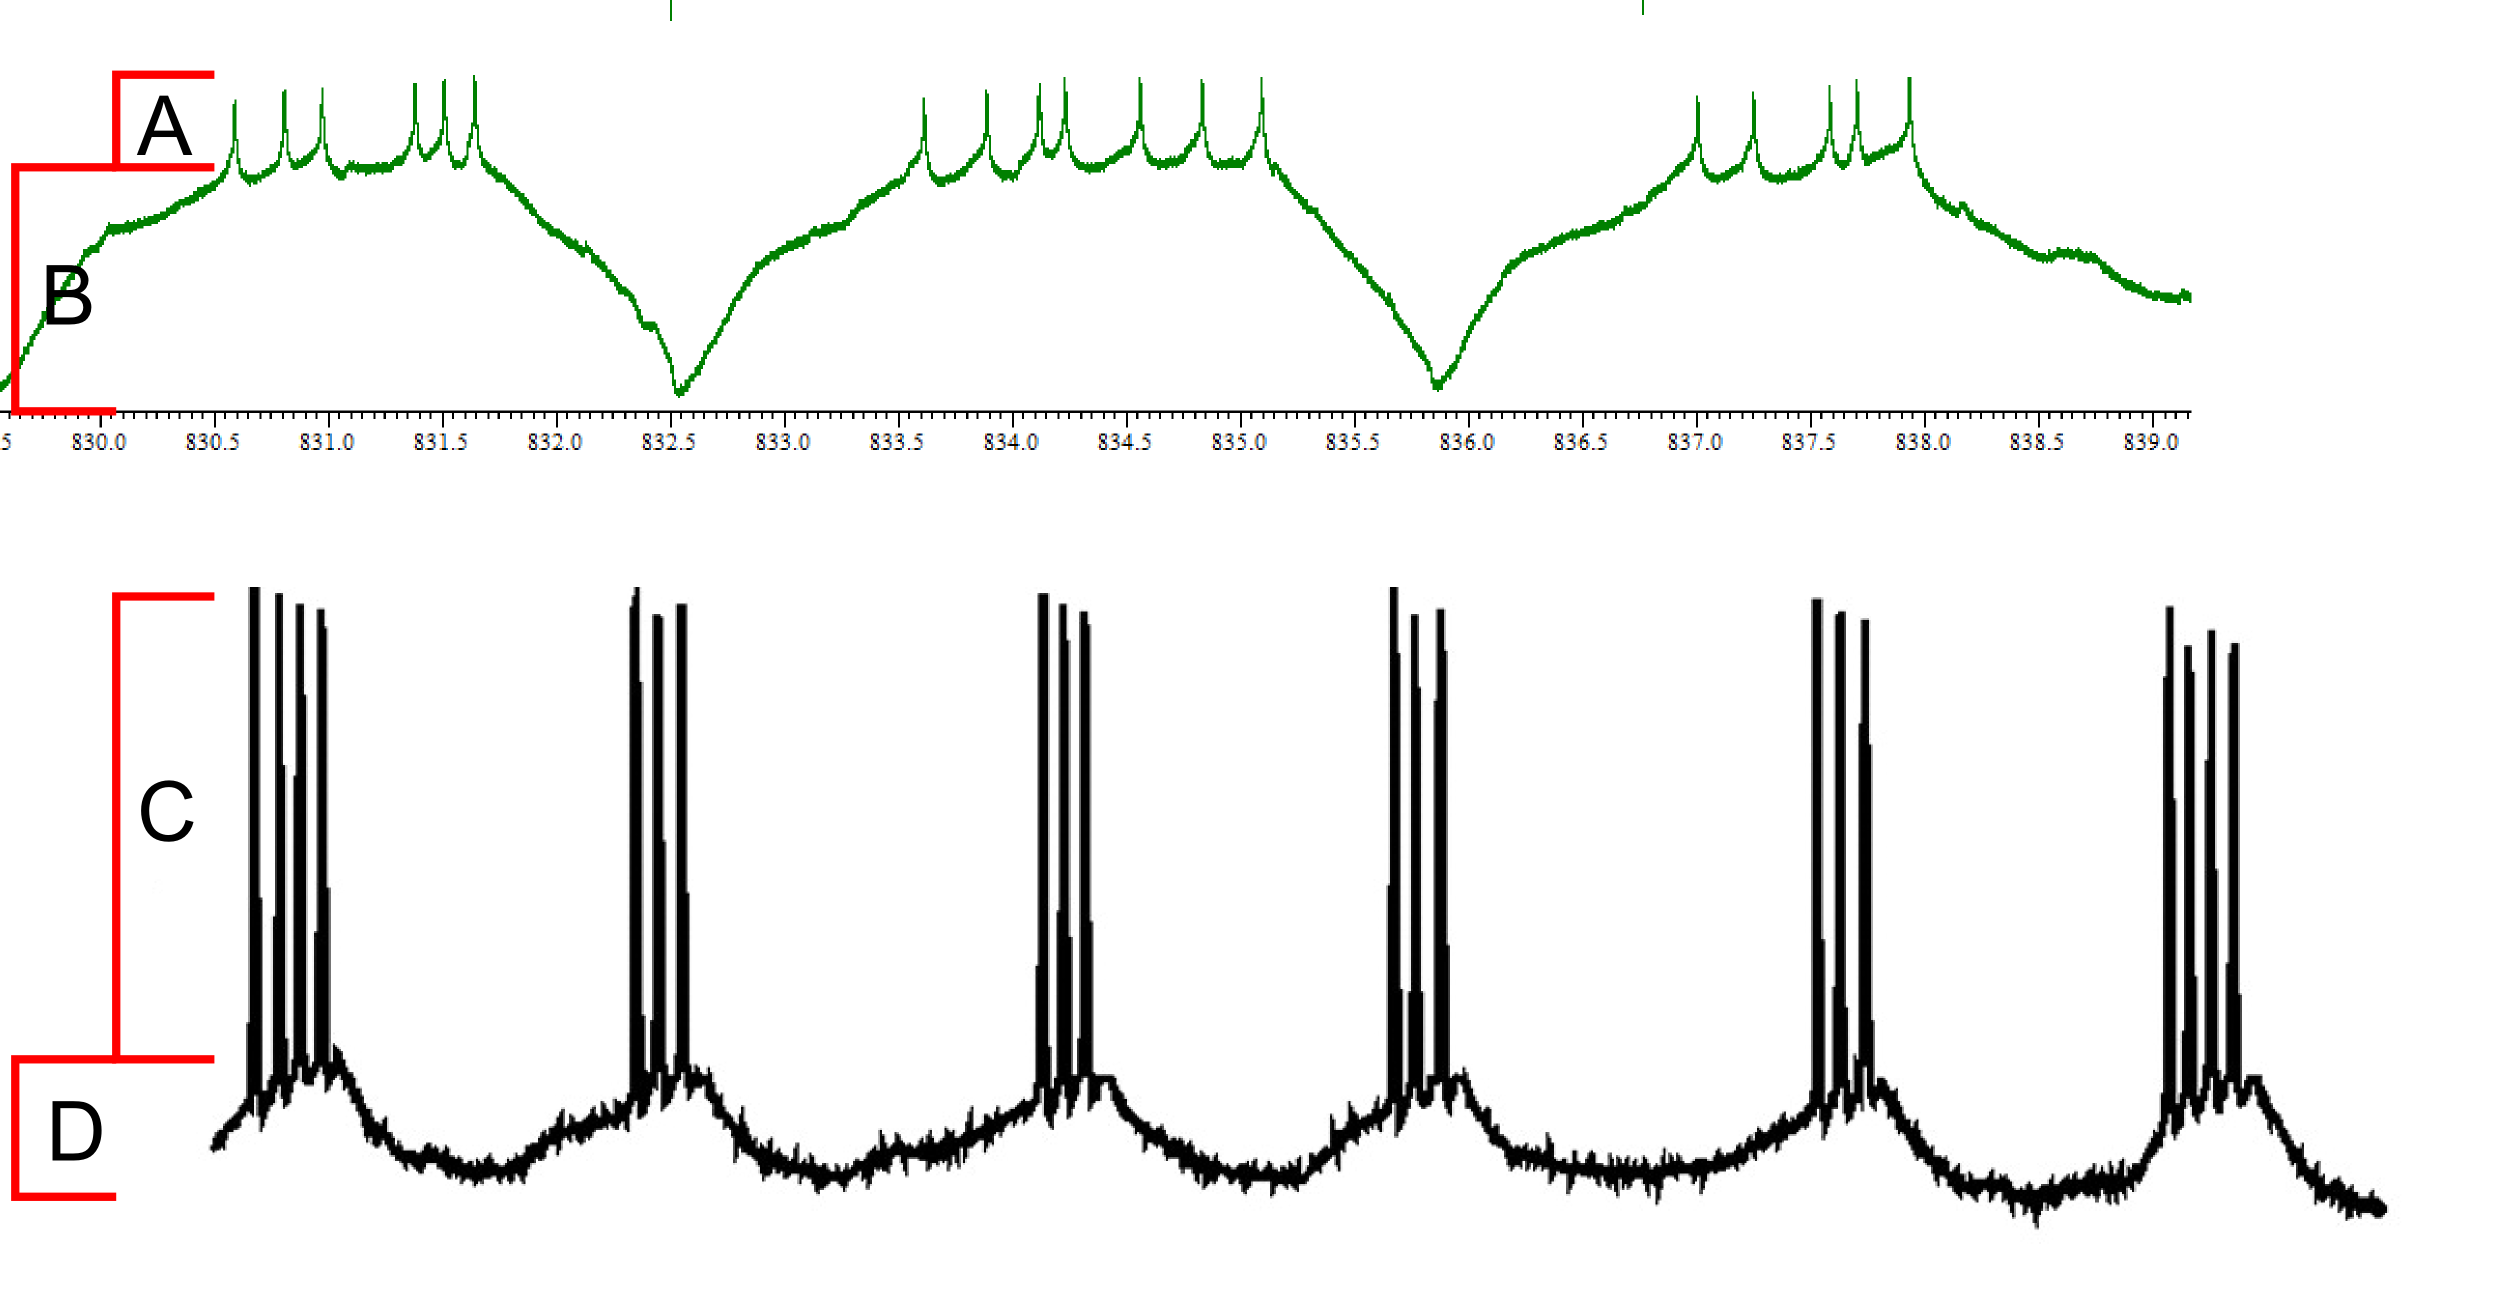
\includegraphics[width=\columnwidth]{graphics/Spikes_comparison.png}
		\caption[Comparison of mammalian and invertebrate neural spikes. ]{\textbf{Comparison of mammalian and invertebrate neural spikes.} The trace at the top is an intracellular recording of a neuron in the crab stomatogastric ganglion. Typical of invertebrate spikes, the amplitude of the spikes (A) is smaller than the depolarisation amplitude of the plateau (B). In the case of mammalian spikes, the amplitude of the spikes (C) are much larger than the amplitude of the plateau (D). (Mammalian spikes from \cite{Wang1999}.)}
		\label{fig:spike_comparison}
	\end{center}
\end{figure}
%\note{\cite{Wang1999,Wang2010,Gray1996}}

In general the change in the relative temporal ordering of the activity of multiple neurons is reflected by changes in the relative timing of individual spikes or bursts of spikes generated by these neurons. Thus, the temporal dynamics of relative activities of neurons is reflected also by the dynamics of the relative timing of activity plateaus of these neurons.

In the case of micro-electrode intra-cellular recording of neurons individual spikes, even as part of a burst of spikes, can easily be distinguished. In the case of optical imaging recording of neural activities, this is often not the case due to inherent noise of imaging. This means that relying on the determination of spike and burst times of individual neurons is relatively difficult and the use of these neural activity markers is relatively unreliable for the estimation of the dynamics of the temporal relationships of the neural activities.

In this section, the use of the timing of the activity plateaus of neurons for the estimation of the dynamics of the temporal relationships of their activities is proposed. The proposed heuristic analysis works off-line, following the recording of the activity of the neurons. In order to use activity plateaus for this purpose a set of salient features of these that can be determined robustly using the noisy optical imaging data needs to be defined. Given that, in general, the activity plateaus are preceded by a ramp-up phase and are followed by a ramp-down phase of the membrane potential in the soma of the neuron, the salient features of neural activity profile that are chosen are indicators of the timing of the ramp-up, ramp-down and the beginning and ending of the plateau itself (fig \ref{fig:activity_profile}).

\begin{figure}[H]
	\begin{center}
		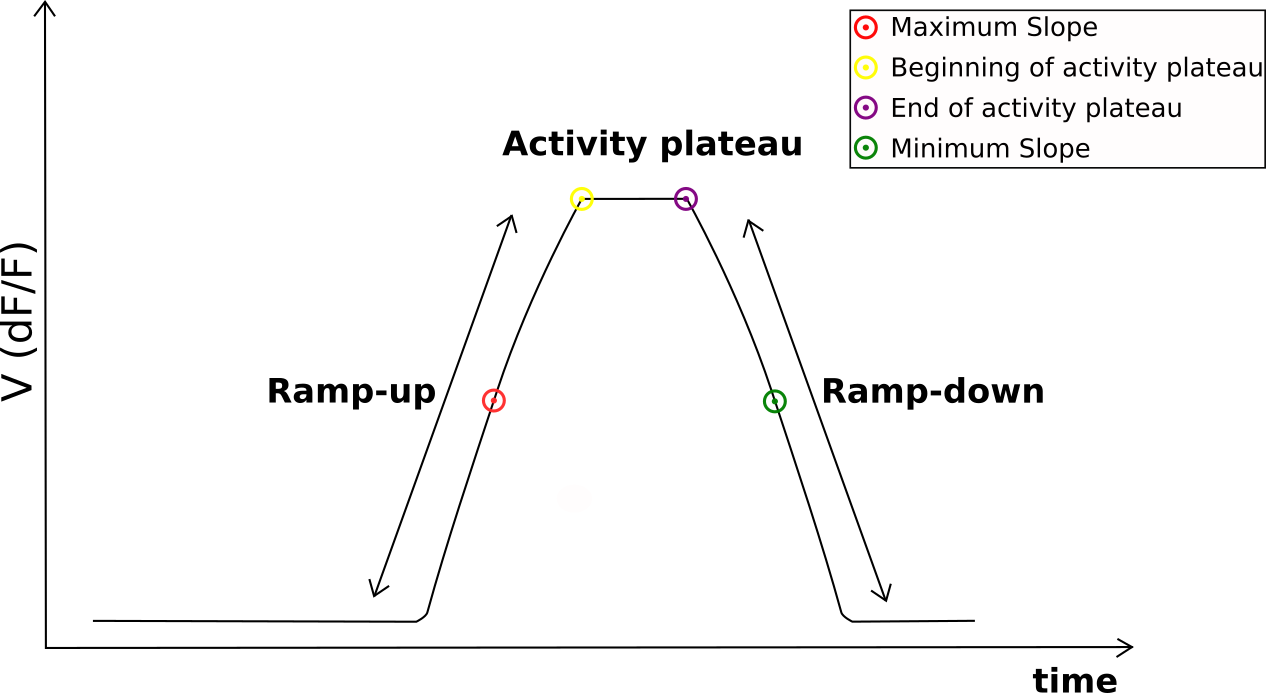
\includegraphics[width=\columnwidth]{graphics/activity_profile.png}
		\caption[Typical activity profile of a neuron.]{\textbf{Typical activity profile of a neuron.} The spiking happens during the activity plateau, which is preceded by the ramp-up phase and followed by the ramp-down phase. The vertical axis shows the membrane potential of the neuron.}
		\label{fig:activity_profile}
	\end{center}
\end{figure}

To find the timing of the ramp-up phase, the time point for which the upward slope of the neural activity profile is maximal is numerically determined. An appropriate time interval that lasts for around the usual duration of the measured ramp-up phases has to be chosen. This point is expected to be around the mid-point of the ramp-up phase. To find the \textbf{\textit{maximum upward slope point}} (or maximum slope point, given that the upward slope is a positive slope), the slope of the best linear approximation of the data points representing the neuron's activity profile for an appropriately chosen time window centred on the time of the given time step is calculated for each step. Assuming that $x_{t}$ are the measured values of the neural activity at recording time step $t$, it means that time intervals of $2\tau+1$ measurement time units is considered and the \textbf{\textit{local slope approximation}} $m_{t}$ is calculated such that:

\begin{equation}
\label{eq:local_slope}
(m_{t},b_{t})=\frac{argmin}{m,b}\sum^{t+\tau}_{u=t-\tau}(x_{t}-m\cdot(u-t+\tau)-b)^2
\end{equation}

The maximum slope point for a time interval $[T_{1},T_{2}]$, measured in units of recording time steps, is the point on the activity profile of the neuron corresponding to the time point $t^{*}$ for which 

\begin{equation}
m_{t^{*}}=\max_{t\in[T_{1},T_{2}]}m_{t}
\end{equation}

If the time interval $[T_{1},T_{2}]$ is chosen such that $T_{2}-T_{1}$ is approximately the usual time length of the ramp up phase (measure in units of recording time steps) and $\tau$ is chosen appropriately (e.g. $\tau=(T_{2}-T_{1})/2$ or slightly less), then it can be expected that the above calculation will find the maximum slope point of the neural activity profile corresponding to the time interval $[T_{1},T_{2}]$. If the chosen time interval is such that during this time interval the neuron's activity profile follows a ramp-up phase, the maximum slope point that is found is likely to indicate the midpoint of the ramp-up phase. If the chosen interval is such that the activity profile of the neuron for this interval does not match a ramp-up phase, the maximum slope point that is found will not indicate the mid-point of a ramp-up phase. Such points are called \textbf{\textit{spurious maximum slope points}}.

To distinguish between maximum slope points which indicate valid mid-points of ramp-up phases and those which do not, the value ranges of the calculated maximum slope values for many considered time intervals have to be considered. If the membrane potential variation associated with the ramp-up phase is larger than the membrane potential variation associated with spikes measured in the neuron soma, the slope values for valid maximum slope points will be much larger than the slope values calculated for spurious maximum slope points.

In general, spurious maximum slope points, calculated for periods of relative silence of neural activity, will have small maximum slope values associated with them (possibly very close to zero). If the soma membrane potential variations associated with spikes are larger than the soma membrane potential variation during the ramp-up phase, some spurious maximum slope points may have larger slope values associated with them than the slope values calculated for valid maximum slope points. In such cases it is necessary to rely on setting the appropriate and sufficiently narrow value interval for valid maximum slope values based on the analysis of the experimental data. Figure \ref{fig:slopes} presents synthetic examples of these two cases demonstrating the determination of the maximum slope points.

\begin{figure}[H]
	\begin{center}
		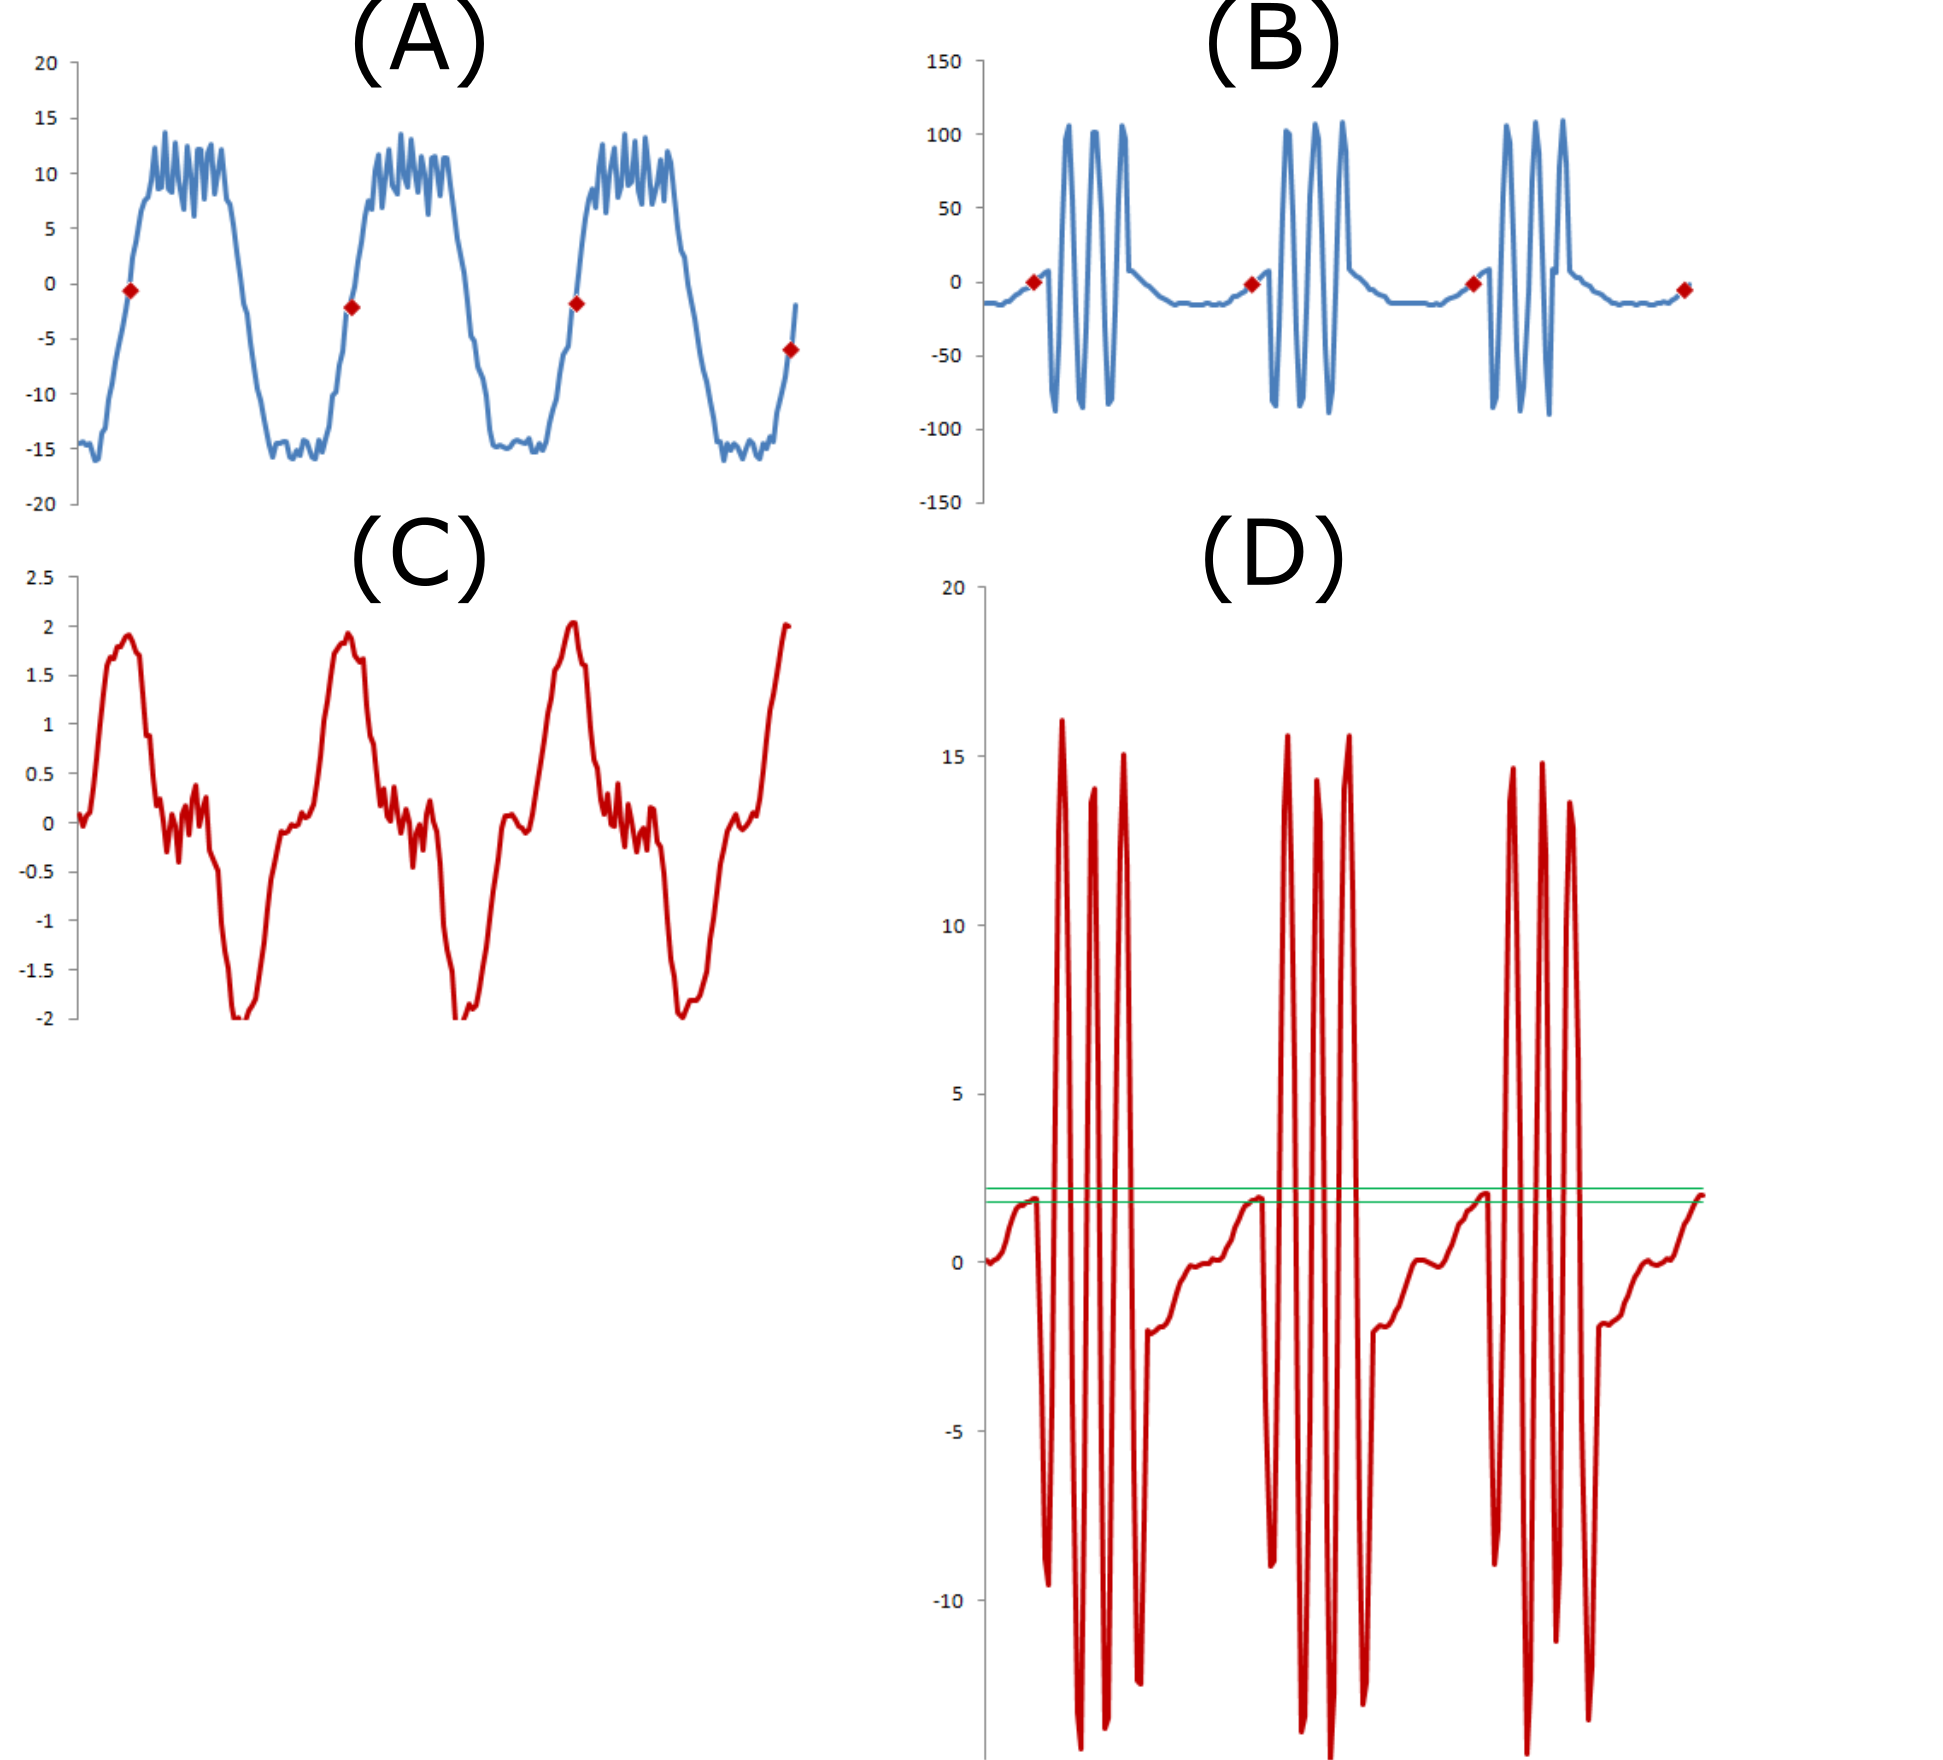
\includegraphics[width=\columnwidth]{graphics/slopes.png}
		\caption[Calculating maximum and local slopes. ]{\textbf{Calculating maximum and local slopes. }(A) Maximum slope points calculated for simulated neural activity having a plateau potential difference that is much larger than the potential difference corresponding to spike activity; (B) The calculated local slope values for the data shown in (A); (C) Maximum slope points calculated for simulated neural activity having a plateau potential difference that is much smaller than the potential difference corresponding to spiking activity; (D) The calculated local slope values for the data shown in (C). The horizontal axis is always time, the vertical axis represents the voltage in (A) and (C) in arbitrary units and the local slope value (B) and (D).}
		\label{fig:slopes}
	\end{center}
\end{figure}

For the timing of the ramp-down phase the time point with the maximal downward slope of the neural activity profile is determined. A method, similar to that used for determining of the maximum slope point is used. In the case of the ramp-down phase the general expectation is that the minimum slope (equivalent to the maximum downward slope) point is around the middle of the ramp-down phase. To find the minimum slope point the calculation for each time stop of the slope of the best linear approximation of the data points representing the neuron's activity profile for an appropriate time window centred on the given time step (Eq.\ref{eq:local_slope}) is used. The minimum slope point for a time interval $[T_{1},T_{2}]$ measured in units of recording time steps is the point on the activity profile of the neuron corresponding to the time point $t^{**}$ for which:

\begin{equation}
\label{eq:min_slope_point}
m_{t^{**}}=\min_{t\in[T_{1},T_{2}]}m_{t}
\end{equation}

As stated previously, for approximately chosen $T_{2}-T_{1}$ and $\tau$ it can be expected that equation \ref{eq:min_slope_point} finds the minimum slope point of the neural activity profile corresponding to the time interval $[T_{1},T_{2}]$. If the chosen interval is such that the activity profile of the neuron for this interval does not match a ramp-down phase, the minimum slope point that is found will not indicate the mid-point of a ramp-down phase, and these are called \textbf{\textit{spurious minimum slope points}} points, similarly to spurious maximum slope points. As in the case of maximum slope points, if the membrane potential change associated with the ramp-down phase is considerably larger than the soma membrane potential change associated with spikes, the valid minimum slope points will be significantly smaller than the spurious minimum slope points, which are expected to have values close to zero. If the membrane potential changes in the soma associated with spikes are larger than the membrane potential change of the ramp-down phase, the determination of the valid minimum slope points relies on the experimental determination of the acceptability range of valid minimum slope values and those minimum slope points are considered valid for which the associated slope value is in this acceptability range.

In the case of neurons with large change of membrane potential difference during ramp-up and ramp-down phases and relatively small changes of the membrane potential difference during the spikes, the calculation of local slope approximation also allows the estimation of the beginning and the end of the activity plateau. The estimation cannot be done reliably for neurons where the membrane potential difference changes in the soma during spiking are much larger than the changes during the ramp-up and ramp-down phases.

To find the estimated points for the beginning and the end of the activity plateau the local forward and backward slopes of the neural activity are considered. The \textbf{\textit{local forward slope}}, at a time point, is the slope of the best linear approximation of the neural activity starting from that time point and for some time period forward. It is expected that the local forward slope gets close to zero around the start of the activity plateau, given that the soma membrane potential difference variations related to spikes are relatively small, and that the local forward slope is considerably positive for time points before the start of the activity plateau. Similarly, the \textbf{\textit{local backward slope}} at a time point is the slope of the best linear approximation of the neural activity over some time period ending at this  time point. In general, it can be expected that the local backward slope is close to zero for time points on the activity plateau and becomes considerably negative as the activity of the neurons goes into the ramp-down phase. So, the end of the activity plateau is indicated by the last time point where the local backward slope is close to zero.The estimated local forward and backward slope, $m_{t}^{f}$ and $m_{t}^{b}$ respectively, are calculated as follows:

\begin{equation}
\label{eq:forward_slope}
(m_{t}^{f},b_{t}^{f}) = \frac{argmin}{m,b}\sum_{u=t}^{t+2\tau}(x_{t}-m\cdot(u-t+\tau)-b)^{2}
\end{equation}

\begin{equation}
\label{eq:backward_slope}
(m_{t}^{b},b_{t}^{b}) = \frac{argmin}{m,b}\sum_{u=t-2\tau}^{t}(x_{t}-m\cdot(u-t+\tau)-b)^{2}
\end{equation}

Next, the points on the activity profile of the neuron for which the calculated local forward and backward slope values are close to zero have to be found. The acceptable range of close to zero values may be determined on a case-by-case basis examining the calculated slope values. In principle the acceptability range may be chosen as $[-\epsilon \cdot m_{max},\epsilon \cdot m_{max}]$, where $m_{max}$ is the maximal absolute value of the calculated slope values associated with maximum and minimum slope points and $\epsilon$ is a small number, for example $\epsilon=0.1$. This range of values is called the \textbf{\textit{zero value range}} and is denoted as $[-z^{*},z^{*}]$. Following the finding of all the points with forward and backward slope values within the zero value range the first of these that follows a maximum slope point and the last that precedes the minimum slope point are determined. These two points will be estimates of the beginning and the end, respectively, of the \textbf{\textit{activity plateau}} of the neuron. In formal terms it is determined as:

\begin{equation}
\label{eq:plateau_begin}
T^{z,f} = \{t|m_{t}^{f} \in [-z^{*},z^{*}]\}
\end{equation}

\begin{equation}
\label{eq:plateau_end}
T^{z,b} = \{t|m_{t}^{b} \in [-z^{*},z^{*}]\}
\end{equation}

then $t_{b}^{0}$ and $t_{e}^{0}$ are determined such that:

\begin{equation}
\label{eq:plateau_time_begin}
t_{b}^{0} > t^{*}, t_{b}^{0} \in T^{z,f},t_{b}^{0} \leq t, \forall t \in T^{z,f},t>t^{*}
\end{equation}

\begin{equation}
\label{eq:plateau_time_end}
t_{e}^{0} > t^{*}, t_{e}^{0} \in T^{z,b},t_{b}^{0} \leq t, \forall t \in T^{z,b},t<t^{*}
\end{equation}

The beginning and end of the activity plateau will be the points corresponding to the time steps $t_{b}^{0}$ and $t_{e}^{0}$ respectively. In general, it should be possible to determine an activity plateau for each consecutive  pair of maximal and  minimal slope points. Figure \ref{fig:min_max_points} exemplifies the determination of maximum and minimum slope points and the beginning and end points of activity plateaus using synthetic data for a neuron with large membrane potential difference changes associated with ramp-up and ramp-down phases and relatively small such changes in the soma associated with spikes.

\begin{figure}[H]
	\begin{center}
		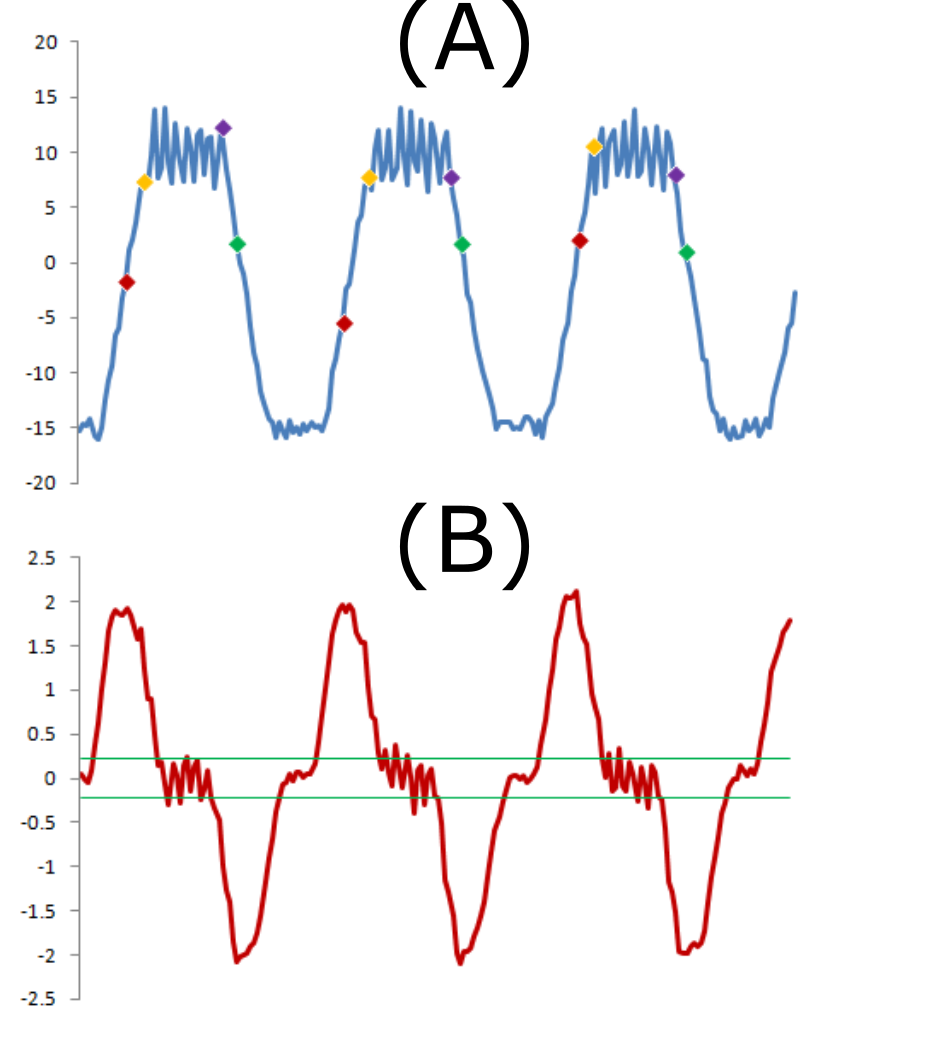
\includegraphics[width=\columnwidth]{graphics/min_max.png}
		\caption[Finding the activity plateau.]{\textbf{Finding the activity plateau.} (A) Simulated activity of a neuron. The \textbf{calculated maximum slopes} are shown as red dots and the \textbf{calculated minimum slopes} are shown as green dots. The beginning  and end points of activity plateaus are shown with yellow and purple dots respectively; (B) The thin green lines indicate the value band that is considered to correspond to the activity plateau following the maximum slope point. The horizontal axis is time in both cases,  while the vertical axis represents voltage in (A) in arbitrary units and the calculated local slope value in (B).}
		\label{fig:min_max_points}
	\end{center}
\end{figure}

Following the determination of maximum and minimum slope points and possibly of the beginning and end points of activity plateaus for multiple neurons recorded simultaneously the timing of these points can be used to analyse the changes in the temporal relationship of the activities of the recorded neurons. Depending on the number of the kinds of salient points determined, multiple estimates about the observable temporal features of the joint activity of the considered neurons can be obtained. For example, the average time difference between maximum slope points of the two rhythmically active neurons indicates the temporal difference between the activation of the neurons, while the average time difference between minimum slope points of the same neurons indicates the temporal difference between the inactivation of these neurons. Phase locking between the neurons is indicated by small standard deviations of  the calculated temporal differences between matching maximum slope or minimum slope points of the neurons and the relaxation of phase locking is implied by an increase of the standard deviation for example following exposure to a neuromodulator.

The robustness of the above proposed calculations can be assessed by considering $x_{t} = \tilde{x}_{t}+z_{t}$, where $\tilde{x}_{t}$ is the true value of the membrane potential difference and $z_{t}$ is an additive noise with zero mean and $\sigma$ standard deviation. Considering the formula (Eq. \ref{eq:local_slope}) for the local slope (a similar approach applies for the local forward and backwards slopes as well), following algebraic manipulation we find that:

\begin{equation}
\label{eq:ten}
m_{t}=\frac{3}{\tau(\tau+1)(2\tau + 1)}\cdot \sum_{u=t-\tau}^{t+\tau}(u-t) \cdot x_{u}
\end{equation}

Considering the composition of $x_{t}$ leads to:

\begin{equation}
\label{eq:eleven}
m_{t} = \tilde{m}_{t} + \mu_{t}
\end{equation}

where $\tilde{m}_{t}$ is the correct local slope value and $\mu_{t}$ is an additive noise in the estimate of the by $m_{t}$. For $\mu$ we get that:

\begin{equation}
\label{eq:twelve}
\mu_{t} = \frac{3}{\tau(\tau + 1)(2\tau + 1)}\cdot \sum_{u=-\tau}^{\tau}u \cdot z_{u+t}
\end{equation}

\begin{equation}
\label{eq:thirteen}
\sigma_{\mu_{t}}^{2} = \frac{9}{(\tau(\tau+1)(2\tau+1))^2}\cdot \sum_{u=-\tau}^{\tau}u^{2} \cdot \sigma^{2} = \frac{3\sigma^{2}}{\tau(\tau+1)(2\tau+2)}
\end{equation}

and

\begin{equation}
\label{eq:fourteen}
\bar{\mu_{t}} = 0
\end{equation}

Thus, the additive noise in the estimates of the local slope follows a normal distribution with zero mean and standard deviation equal to:

$\sqrt{\frac{3}{\tau(\tau+1)(2\tau+1)}}\cdot\sigma$.

In comparison, if the aim is to detect the presence of spikes in the recorded neural activity data, a simple way is to compare the value of the recording to the local average value of the recordings, and conclude the presence of the spike if the difference between the compared values is sufficiently large. In this case the comparison is based on the local average activity value; 

$\bar{x_{t}} = \frac{1}{2\tau+1}\cdot\sum_{u=t-\tau}^{t+\tau}x_{u}$

for which the contained additive noise has zero mean and a standard deviation equal to $\sqrt{\frac{1}{(s\tau+1)}}\cdot\sigma$. Consequently, the likely errors affecting this approach will be larger than the estimation errors affecting our proposed methodology since $\sqrt{\frac{3}{\tau(\tau+1)(2\tau+1)}}\cdot\sigma<\sqrt{\frac{1}{(2\tau+1)}}\cdot$ for $\tau>1$.

\section{Results}
\label{subsec:application}

The proposed methodology (section \ref{sec:analysis_methods}) is demonstrated here by analysing data recorded from dyed \ac{PY} neurons in the crab \ac{STG}. For each \ac{PY} cell the recordings contain between 50 to 80 full activity patterns, each corresponding to a pyloric rhythm cycle. Figure \ref{fig:vsd_recording} shows a sample of the recordings including the identified maximum and minimum slope points and beginning and end points of activity plateaus for the recorded PY neurons. To quantify the effect of dopamine on the synchronisation of the \ac{PY} neurons the temporal delays between corresponding maximum and minimum slope points and beginning and end points of activity plateaus of pairs of \ac{PY} neurons were measured. The mean values and standard deviations of the temporal delays were calculated. 

\begin{figure}[H]
	\begin{center}
		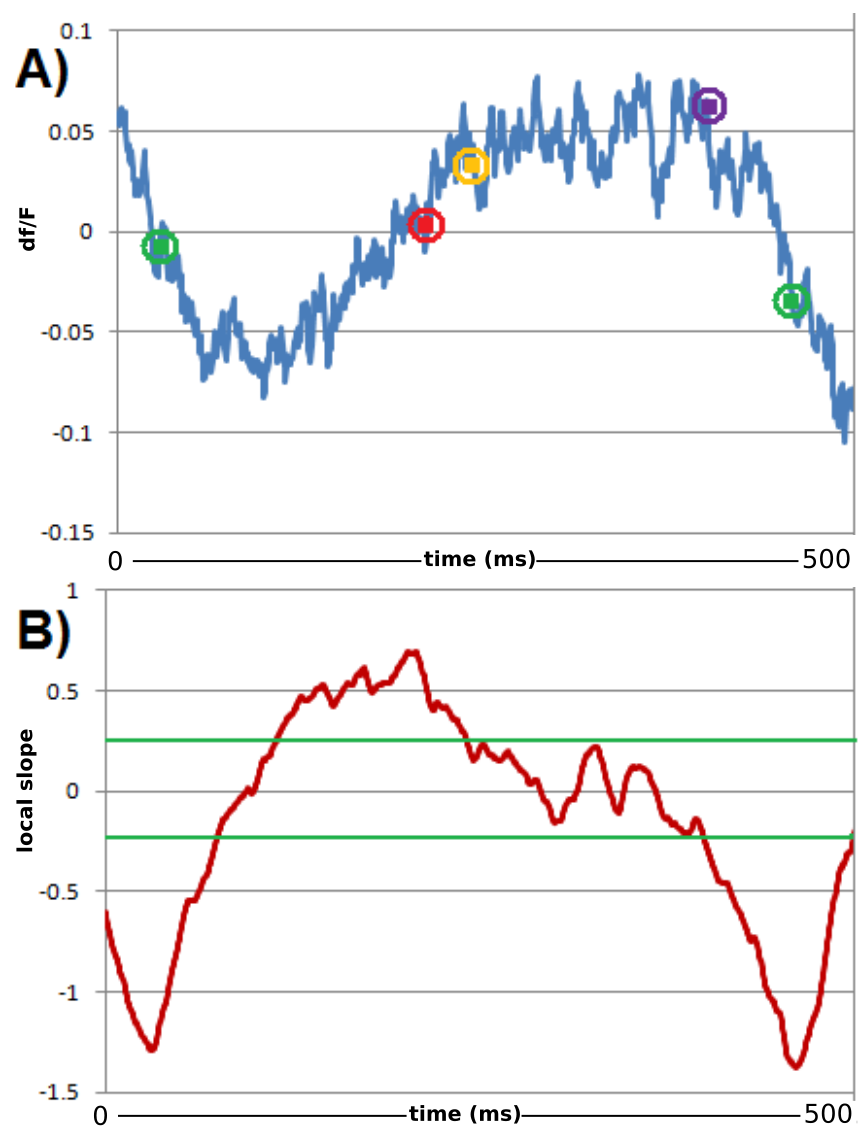
\includegraphics[width=\columnwidth]{graphics/vsd_recording.png}
		\caption[Calculated salient features shown on \ac{VSD} recording.]{\textbf{Calculated salient features shown on \ac{VSD} recording.} \Acp{VSD} recording of a PY neuron together with the minimum (green) and maximum slope (red) points and beginning (yellow) and end (purple) points  of the activity plateau determined from the data; B) The calculated local slope values, the green horizontal lines indicate the band of values considered to correspond to the activity plateau following the maximum local slope point. The horizontal axis is time in both cases and the vertical axis is voltage in arbitrary units in A) and the local slope value in B).}
		\label{fig:vsd_recording}
	\end{center}
\end{figure}

In total 11 pairs of \ac{PY} neurons from four \ac{STG} preparations (two using dye filling and two using bath application of the dye) were considered (see table \ref{tab:experiments}). The mean values and standard deviations of the temporal delays were calculated. It was found that the standard deviation of the temporal delays changed significantly in half of the cases (according to the F-test) following the application of the \ac{DA} containing saline. Results are shown in table \ref{tab:da_results} and figure \ref{fig:da_results}. In 22 cases of 44 comparisons of standard deviations it was found that the standard deviations are significantly larger following the effect of the \ac{DA} on the neurons. In one case it was found that the calculated standard deviation was significantly lower following the \ac{DA} exposure, and in the remaining 21 cases the difference between the standard deviations was not statistically significant. The lack of statistical significance means that the exposure to \ac{DA} did not have an effect on the standard deviation of temporal differences between the corresponding maximum and minimum slope points and beginning and end points of activity plateaus of pairs of \acp{PY}. The increase of the standard deviation of the temporal differences implies reduction of the temporal locking of the \acp{PY}, or in other words, the de-synchronisation of \acp{PY}. The expectation of the de-synchronisation effect of \ac{DA} on the \acp{PY} is thus confirmed.

\begin{table}
	\small
	\caption[Neuron pair comparisons.]{\textbf{Neuron pair comparisons.} In total 11 pairs of \ac{PY} neurons from four \ac{STG} preparations were considered. Two experiments used dye filling and two were bath applications. For each experiment the neurons were compared under control and \ac{DA} conditions. Using the F-test a p-value was obtained for each of the four features, thus giving the 44 values as in table \ref{tab:da_results}}.
	\label{tab:experiments}
	\begin{tabular}{llll}
		\hline
		\textbf{Experiment} & \textbf{Comparison 1} & \textbf{Comparison 2} & \textbf{Comparison 3} \\ 
		\hline
		1 (dye filling) & PY1 with PY2 & - &PY2 with PY3\\
		2 (dye filling) & PY1 with PY2 & PY1 with PY3 &PY2 with PY3\\
		3 (bath application) & PY1 with PY2 & PY1 with PY3 &PY2 with PY3 \\
		4 (bath application) & PY1 with PY2 & PY1 with PY3 &PY2 with PY3 \\
		
		\hline
	\end{tabular}
\end{table}

The suggested approach offers a way to quantify the extent of de-synchronisation of \acp{PY} in response to exposure to \ac{DA}. The presented analysis of \acp{PY} demonstrates that the methodology proposed, can be applied successfully to analyse the dynamics of temporal relationships of neural activities using optical imaging data.

\begin{table}[H]
	\small
	\centering
	\caption[Results of the \ac{DA} experiments.]{\textbf{Results of the \ac{DA} experiments.} p-values of the F-test comparisons of the temporal delay standard deviations. Significant values are shown in red.}
	\label{tab:da_results}
	\begin{tabular}{p{30mm} p{30mm} p{30mm} p{20mm}}
		\hline
		\textbf{Maximum} & \textbf{Minimum} & \textbf{Plateau} & \textbf{Plateau} \\
		\textbf{Slope Points} & \textbf{Slope Points} & \textbf{Begin Points} & \textbf{End Points} \\
		\hline
		
		0.657721015 & 0.936337338 & 0.417005168 &  0.986805014 \\
		\textcolor{red}{0.010577057} & 0.064029034 & 0.097578139 & 0.317799703 \\
		\textcolor{red}{0.000196868} & 0.303675632 & \textcolor{red}{0.066103149} & \textcolor{red}{0.019539292} \\
		\textcolor{red}{2.66550x${10^{-19}}$} & \textcolor{red}{4.10299x${10^{-06}}$} & \textcolor{red}{2.01957x${10^{-15}}$} & \textcolor{red}{0.000686408} \\
		\textcolor{red}{7.86896x${10^{-19}}$} & \textcolor{red}{9.69148x${10^{-05}}$} & \textcolor{red}{2.93382x${10^{-15}}$} & \textcolor{red}{0.001116038} \\
		\textcolor{red}{2.92339x${10^{-26}}$} & \textcolor{red}{8.04271x${10^{-09}}$} & \textcolor{red}{8.07804x${10^{-27}}$} & \textcolor{red}{3.30665x${10^{-15}}$} \\
		0.729215365 & 0.637028887 & 0.841677533 & 0.687908256 \\
		0.734146578 & 0.411370955 & 0.302637642 & 0.819808126 \\
		\textcolor{red}{6.67436x${10^{-05}}$} & 0.263113108 & \textcolor{red}{0.006803160} & \textcolor{red}{ 0.000531943} \\
		0.665538015 & \textcolor{red}{0.024729645} & 0.976871651 & 0.131110278 \\
		\textcolor{red}{0.018054682} & \textcolor{red}{0.002703960} & 0.285120361 & \textcolor{red}{0.004076710} \\
		\hline
	\end{tabular}
\end{table}

\begin{figure}[H]
	\begin{center}
		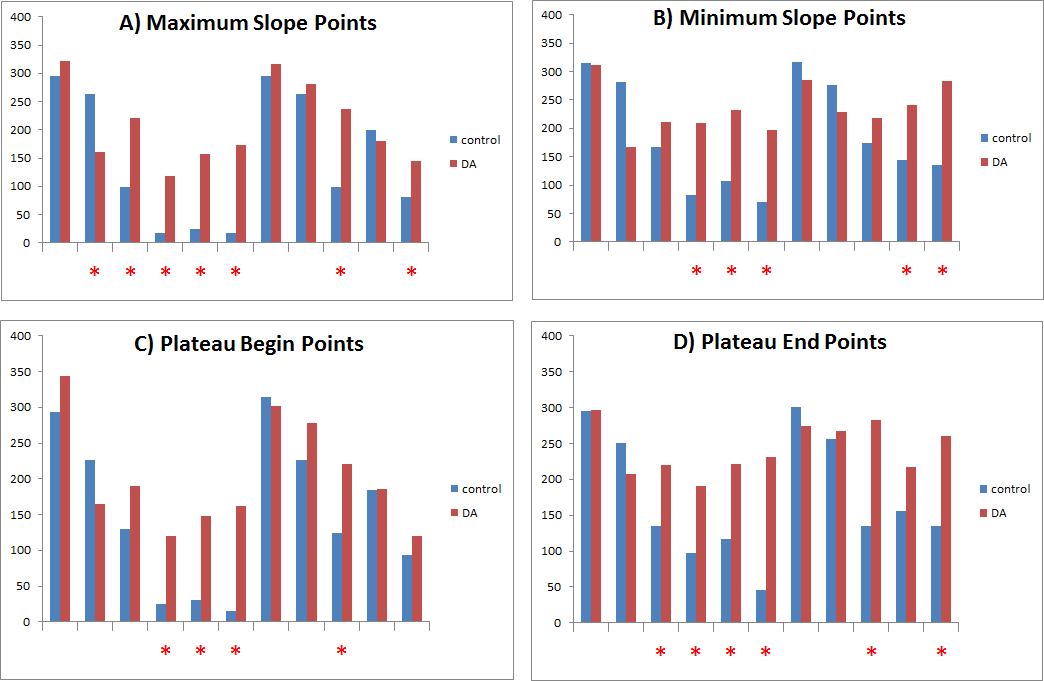
\includegraphics[width=\columnwidth]{graphics/da_results.png}
		\caption[The results of the \ac{DA} experiments.]{\textbf{The results of the \ac{DA} experiments.} The calculated standard deviation values are shown on the vertical axes. Each pair of bars represents a comparison of a pair of \ac{PY} neurons. Comparisons that resulted in a significant p-vale (\textless 0.05) are indicated by a red asterisk on the horizontal axis. The p-values were calculated using the F-test and are given in table \ref{tab:da_results}. PRE indicates standard deviation values calculated before the exposure to dopamine, DA indicates standard deviation values calculated following the exposures to dopamine.}
		\label{fig:da_results}
	\end{center}
\end{figure}

\note{1.7 actual vsd recording of PY neurons. wolfgang 9 may 2011 
	april 2011, 3 data set from aug, sep 2011
	1.8 result of analysis, bar chart showing the effect of the dopamine - the standard deviations are different - using the f-test.}

\section{Discussion and Conclusions}
\label{sec:analysis_discussion}
It is of vital importance that neural circuits are adaptive and flexible in the delivery of their functionality. Such flexibility relies on the dynamics of the temporal relationship between the neurons forming those neural circuits. The recording of many synaptically connected neurons, at individual neuron resolution, has not been possible under physiologically realistic conditions until relatively recently. However, current optical recording techniques using voltage sensitive dyes and calcium dyes allow high spatio-temporal resolution recordings to be made of many neurons.  Such techniques enable us to study the dynamics of temporal relationships of neural activities in biological neural circuits.

In this chapter a method was proposed for the analysis of optical data for understanding the dynamics of the temporal relationship of the activities of individual neurons. The proposed method relies on the robust identification of salient points of the activity patterns of individual neurons, such as the minimum and maximum slope points and the beginning and end points of depolarisation plateaus (the latter two only in appropriate cases). The method is very important because it allows robust analysis of optical neuro-imaging data to determine activity phases of neurons and on the basis of this, allows the quantification and analysis of the dynamics of activity patterns of multiple neurons. Other methods based on the calculation of average measurements are less robust than the method proposed. This kind of analysis is key for the understanding of the emergent functionality of neural systems. Consequently the method proposed here improves the reliability of the use of optical imaging data for this kind of analysis. The proposed method of analysis was applied to neurons recorded in the crab \ac{STG} and it was shown that, as expected, there is a statistically significant, measurable de-synchronisation effect of \ac{DA} on the considered \ac{PY} neurons. This is the first time this effect is shown in the physiologically realistic setting of the \ac{STG}, i.e. previous measurements implying this result were made in the presence of neurotoxic substances to achieve pharmacological isolation of neurons. As noted above the described method is expected to work at best in the case of neurons for which the depolarisation plateau means a larger change in the recorded membrane potential than the spikes themselves. However, it is also expected that the method should work well even for neurons where this is not the case (e.g. neurons of the mammalian cortex). In the case of these neurons the determination of minimum and maximum slope points is feasible and these allow the robust measurement of the dynamics of the temporal relationships of the activity patterns of these neurons using optical imaging data. As shown above, the proposed method works off-line. However, it is possible at least in principle to extend it to an on-line application, if the proposed analysis method is integrated with the recording of the data. With sufficiently fast processors such integration should not represent a major technical challenge. If the method is applied on-line its application is only limited by the time window required for the calculations (consider in particular the case of forward slope calculation), however even this constraint can be mitigated by considering a predictive application of the methodology (e.g. predicting the timing of salient points on the basis of previously
determined salient points and correcting the predictions when the required data becomes available). This kind of on-line application of the methodology would allow setting of additional stimulation of selected neurons depending on the activity pattern phase of measured neurons. This would make possible the design of more elaborated experiments involving measurement and experimental modulation of
the activity of multiple neurons. The method described in this chapter is also applicable to other kinds of noisy biological recordings where robust quantification of key transitions and the measurement of relative transition dynamics across multiple processes is required.
As shown, the calculation of local slope values is more robust than the
calculation of usual averages and this difference in robustness of calculations may be critically important in the context of estimation of activity pattern features from noisy recordings. For example, such cases may include other neural systems (e.g. phase determination of swim pattern generators in leeches or snails) or recordings from muscles (e.g. heart muscles or muscles involved in rhythmic movement or
swimming).

The question now remains whether it is possible to produce a computational model that will reflect the de-synchronisation that was observed. In the next chapter (chapter \ref{chap:modelling}) such a model is discussed. 